% ------------------------------------------------- %
% ---------------------- MOTIVATION ---------------- %
% ------------------------------------------------- %
\section{Motivation}


Modern official statistics operate under a fundamental constraint: survey data ($\mathbf{x}_i, y_i$) is high-signal but expensive and sparse, while administrative, or historical data ($\mathbf{z}_i$) data is ubiquitous and cheap but often suffers from data drift, concept drift, or measurement error. 
Our goal is not merely to impute missing (item non-response), data, but to leverage the ``cheap" frame data ($\mathbf{z}_i$) to reduce the variance of estimates derived from the ``expensive" sample data ($\mathbf{x}_i$), while maintaining robustness against model failure.
% Adding this..to make it clear WE ARE NOT PROPOSING A NEW ESTIMATOR!
Our objective is not to propose a new class of estimators, but to benchmark how existing theoretical frameworks, specifically Model-Calibration and Doubly Robust estimation,perform when applied to the specific constraint of fusing dense historical records with missing current survey data


\begin{figure}[H]
  \centering
  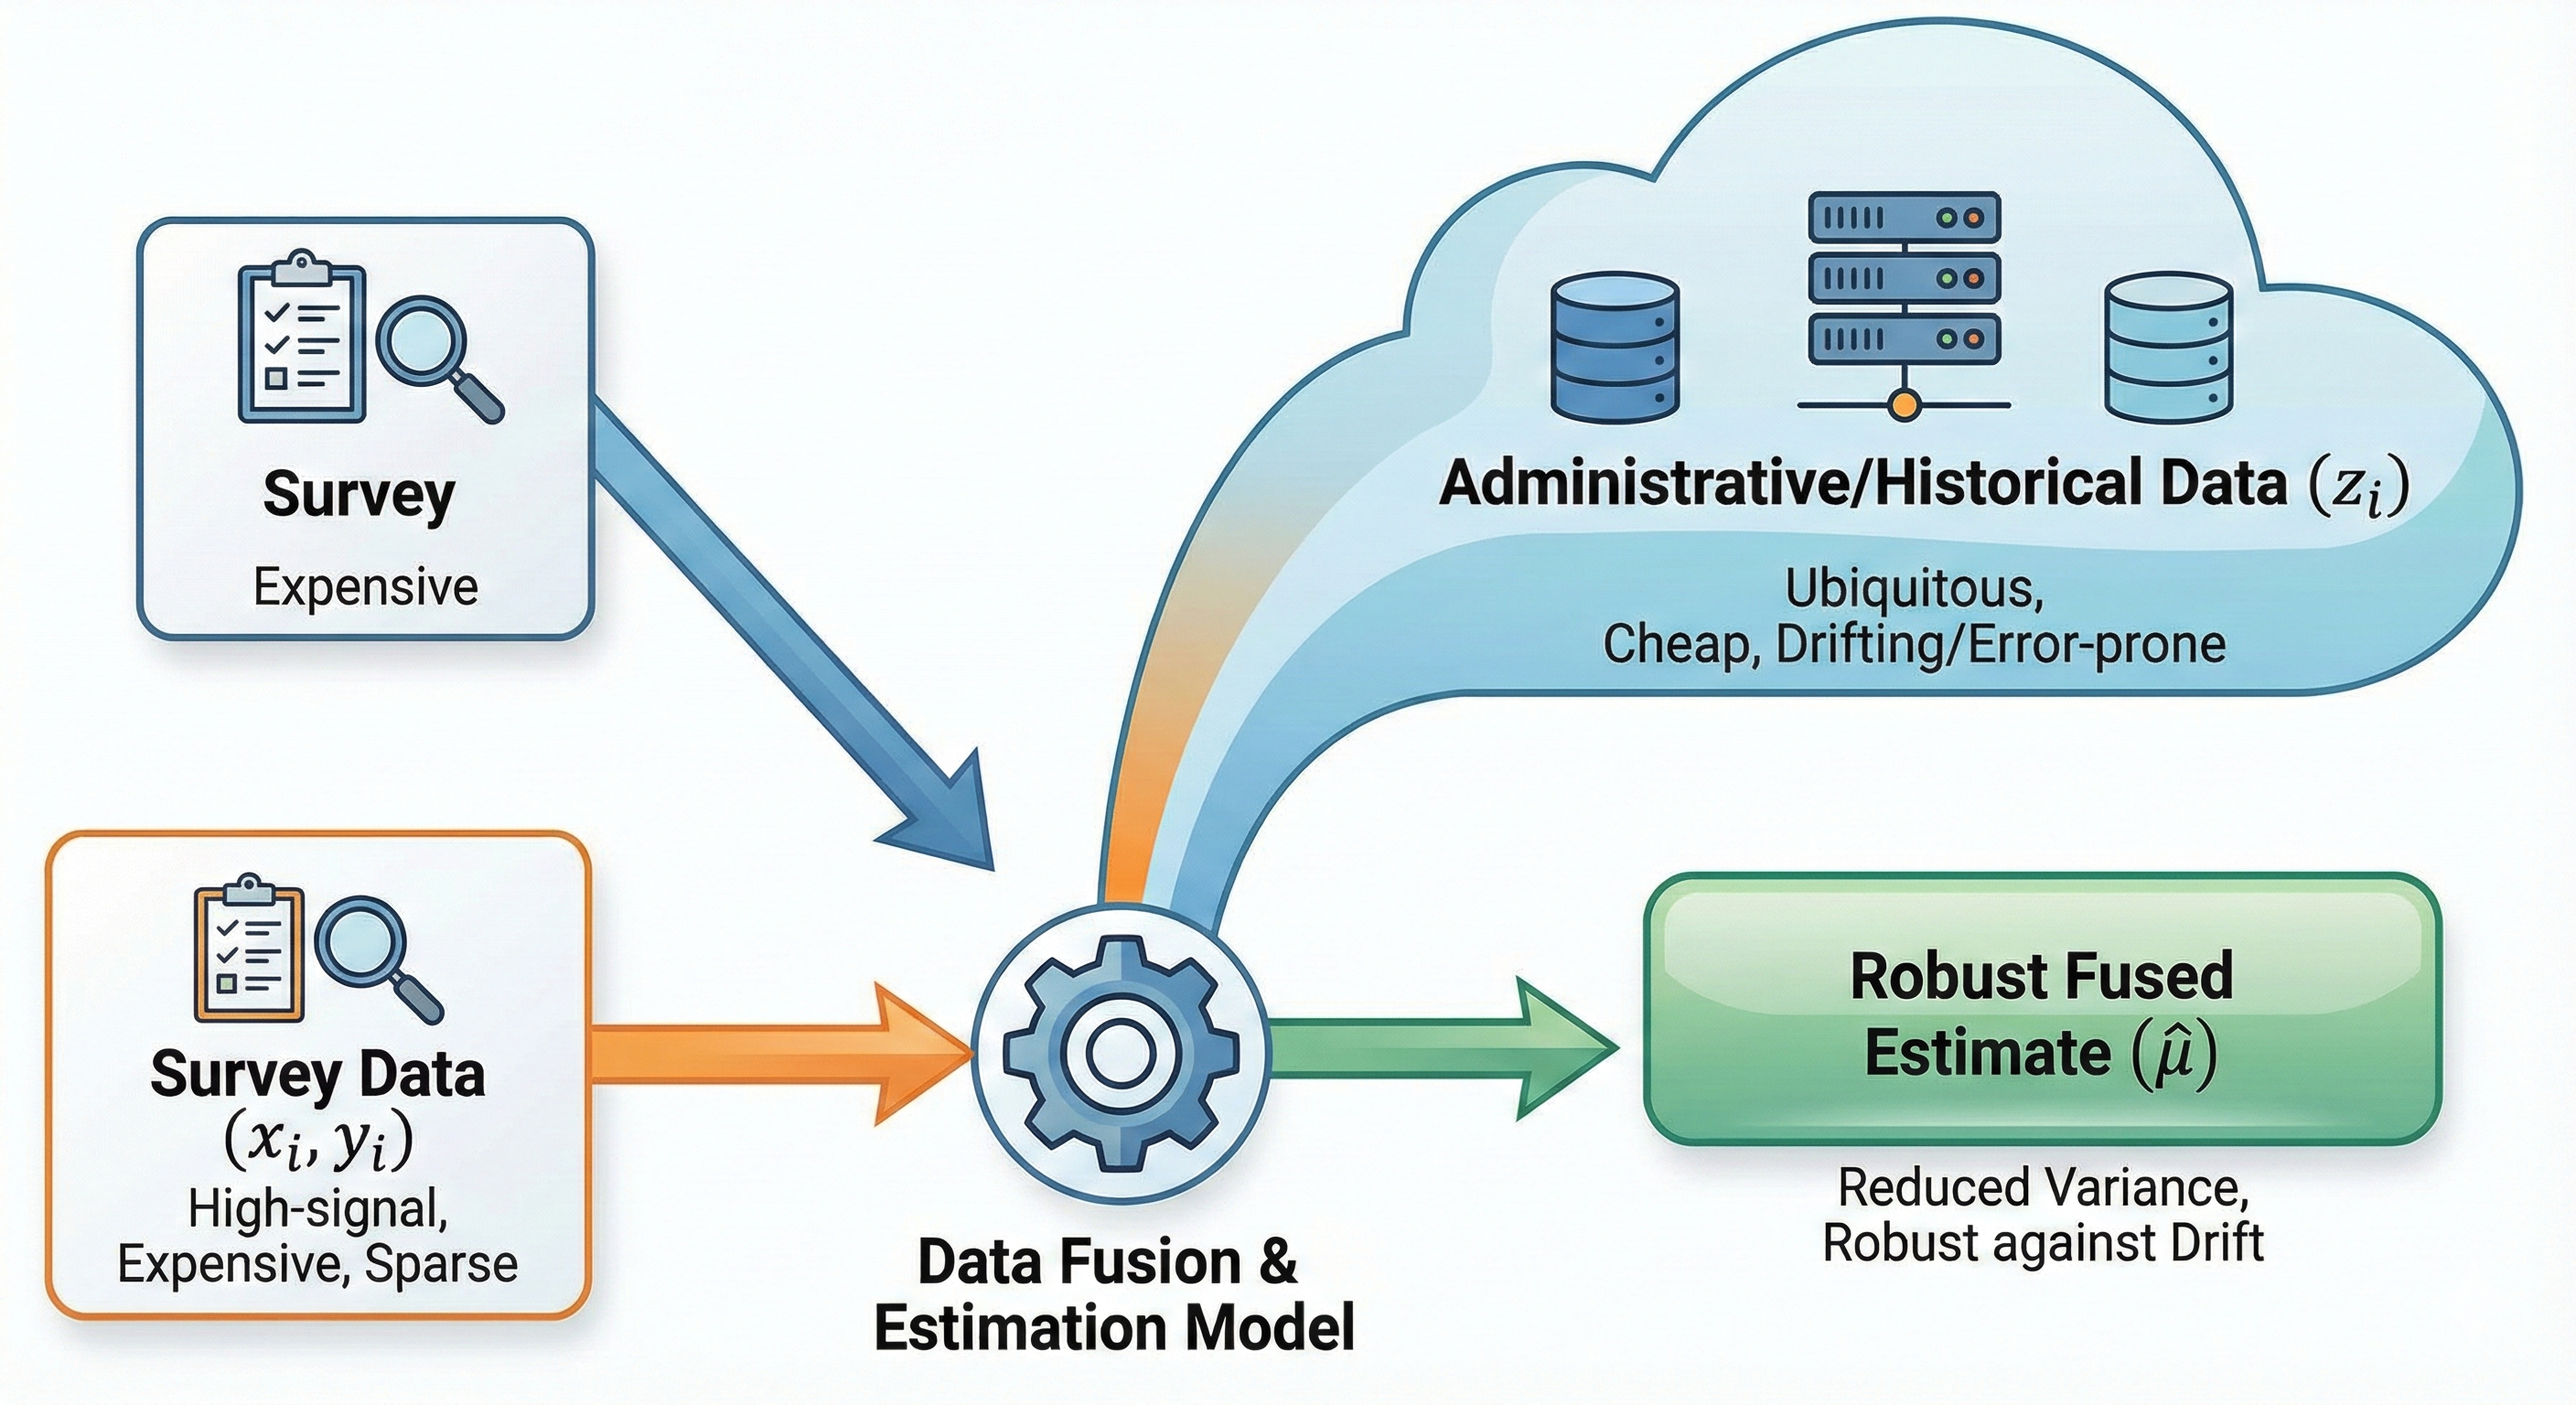
\includegraphics[width=0.8\textwidth]{paper/diagrams/1A.png}
\end{figure}



% ------------------------------------------------- %
% ------------ SCENARIOS OF MISSING DATA ---------- %
% ------------------------------------------------- %
\section{Scenarios of Missing Data}

\begin{itemize}
  \item \textbf{Population ($U$):} Finite population of size $N$, $U=\{1,2,\dots,N\}$.
  \item \textbf{Sample ($S$):} Probability sample of size $n$ drawn from $U$, $S\subseteq U$, $|S|=n$.
  \item \textbf{Inclusion probabilities and weights:} $\pi_i=\Pr(i\in S)>0$ with design weights $d_i:=1/\pi_i$ for $i\in S$. (Second–order probabilities $\pi_{ij}=\Pr(i,j\in S)$ may be defined when needed, assume positive $\pi_{ij}=\Pr(i,j\in S) >0$.)
  \item \textbf{Frame auxiliaries:} $\mathbf{z}_i\in\mathbb{R}^{p_z}$ available for \emph{every} unit $i\in U$.
  \item \textbf{Sample auxiliaries:} $\mathbf{x}_i\in\mathbb{R}^{p_x}$ observed for \emph{all} $i\in S$.
  \item \textbf{Imputation vector:}
    \[
      \mathbf{v}_i :=
      \begin{bmatrix}
        \mathbf{z}_i \\
        \mathbf{x}_i
      \end{bmatrix}
      \in \mathbb{R}^{p_v},
      \qquad p_v = p_z + p_x,
    \]
    used as the predictor set in standard imputation models fit on $S$.


  \item \textbf{Study variable and item indicator (item nonresponse only).}
    Let $q=1$ so $y_i\in\mathbb{R}$. For each $i\in S$, define the \emph{item-response} indicator
    $r_i=\mathbbm{1}\{y_i\ \text{is observed}\}\in\{0,1\}$. The observed value is
    $y_i^{\mathrm{obs}}=r_i\,y_i$. We assume full unit response in this section:
    $R_i\equiv 1$ for all $i\in S$ (no unit nonresponse).
    \item \textbf{Historical Data:} Let $t$ denote the current period. Variables without temporal superscripts refer to the current period: $y_i$, $\mathbf{x}_i$, $\mathbf{z}_i$ are current-period measurements. Historical data from $k$ periods prior are denoted $y_i^{(t-k)}$, $\mathbf{x}_i^{(t-k)}$, $\mathbf{z}_i^{(t-k)}$. In our primary application, we have complete census data (or rich historical surveys) from period $t-1$ and a smaller survey sample from the current period $t$.
    
    \item \textbf{MAR assumption (item nonresponse).}
    Missing at random given predictors $\mathbf v_i=[\mathbf z_i,\mathbf x_i]$:
    for $i\in S$,
    \[
    \Pr(r_i=1 \mid y_i,\mathbf v_i, R_i=1)\;=\;\Pr(r_i=1 \mid \mathbf v_i, R_i=1).
    \]
    Under our “no unit nonresponse” setup ($R_i\equiv 1$), this reduces to
    \[
    \Pr(r_i=1 \mid y_i,\mathbf v_i)\;=\;\Pr(r_i=1 \mid \mathbf v_i).
    \]
    Write $\rho_i:=\Pr(r_i=1\mid \mathbf v_i)$ for the (item) response propensity.

  \item \textbf{Sets and counts:}

      \[
    S_r = \{ i \in S : r_i = 1\}, \qquad
    S_m = \{ i \in S : r_i = 0\}, \qquad
    n_r = \sum_{i \in S} r_i = |S_r|.
    \]
    
\end{itemize}

\noindent\emph{Observed-data summary for each $i\in S$:}
\[
(\, \mathbf{x}_i,\ \mathbf{z}_i,\ \mathbf{v}_i,\ d_i,\ r_i,\ y_i^{\mathrm{obs}}\,), 
\quad\text{with }\mathbf{v}_i=[\mathbf{z}_i,\mathbf{x}_i].
\]
Imputation of missing $y_i$ uses $(y_i^{\mathrm{obs}},\mathbf{v}_i,d_i)$ within $S$; projection estimator uses $f(\mathbf{z}_i)$ for all $i\in U$.



\paragraph{Baseline (Complete Response, Current Period Only)}.

Horvitz-Thompson Estimator:
\[
\hat{\mu}_{\mathrm{HT}}
  = \frac{1}{N} \sum_{i \in S} d_i\, y_i,
  \qquad d_i := \frac{1}{\pi_i}.
\]



Notation: $U$ = population of size $N$; $S \subseteq U$ = sample of size $n$; $\pi_i = P(i \in S)$ = inclusion probability; $y_i$ = study variable for unit $i$.

\paragraph{Scenario 1: Item Nonresponse.}
Now we introduce the scenario where a response variable $y_i$ is missing.
Broadly in the literature, there are three basic approaches to dealing with non-response: Imputation, Re-weighting, and Doubly Robust methods.
Let $r_i = \mathbbm{1}_{\{y_i \text{ observed}\}} \in \{0,1\}$; $S_r = \{i \in S: r_i=1\}$ be the set of respondents; and $S_m = \{i \in S: r_i=0\}$ be the set of missing units. We assume predictors $\mathbf{x}_i$ are available for all $i \in S$.



\medskip
\noindent \textbf{1. Imputation Estimator} (e.g., Kalton and Kasprzyk, 1986; Dagdoug et al., 2025):
This approach predicts missing values using a model $\hat{m}_{S_{r}}(\mathbf{x}_i)$ fit on the respondents.
\[ 
\hat{\mu}_{\text{imp}} = \frac{1}{N}\left(\sum_{i\in S_r}\frac{y_i}{\pi_i} + \sum_{i\in S_m}\frac{\hat{m}_{S_{r}}(\mathbf{x}_i)}{\pi_i}\right) 
\]


where $\hat{m}_{S_{r}}(\mathbf{x}_i)$ is the predicted value from an imputation model fit on respondents $S_r$ for unit $i$ based on predictors $\mathbf{x}_i$.


\medskip
\noindent \textbf{2. Nonresponse Weighting Adjusted (NWA) Estimator} (Oh and Scheuren, 1983; Fay, 1991; Little and Rubin, 2002):
Also known as the Inverse Probability Weighting (IPW) estimator, this approach adjusts the sampling weights by the estimated probability of response, $\hat{p}_i = \widehat{\Pr}(r_i=1 \mid \mathbf{x}_i)$.
\[ 
\hat{\mu}_{\text{NWA}} = \frac{1}{N}\sum_{i\in S_r}\frac{y_i}{\pi_i \hat{p}_i} 
\]


\medskip
\noindent \textbf{3. Doubly Robust (AIPW) Estimator} (Robins et al., 1994; Kim and Haziza, 2014; Haziza and Beaumont, 2017):
This estimator combines the previous two. It uses the imputation model to predict outcomes for the whole sample, and then uses the propensity weights to correct the residuals (the difference between observed and predicted values) for the respondents.
\[ 
\hat{\mu}_{\text{DR}} = \frac{1}{N} \sum_{i \in S} \frac{1}{\pi_i} \left[ \hat{m}_{S_{r}}(\mathbf{x}_i) + \frac{r_i}{\hat{p}_i} \left( y_i - \hat{m}_{S_{r}}(\mathbf{x}_i) \right) \right] 
\]
This estimator is consistent if \textit{either} the imputation model $\hat{m}_{S_{r}}(\cdot)$ \textit{or} the response probability model $\hat{p}_i$ is correctly specified.


\medskip
\noindent An important thing to note here is that in all three cases, we are only using the variables available to us from the sample ($\mathbf{x}_i$). We make no use of additional data that may be available outside of the sample (such as frame data $\mathbf{z}_i$) at this stage.

\paragraph{Scenario 2: Item Nonresponse with Population Auxiliary Data.}

We now extend the previous scenario. In this scenario, we assume access to a vector of auxiliary variables $\mathbf{z}_i$ for every unit in the population $U$ (e.g., census data or administrative records), in addition to sample-specific information $\mathbf{x}_i$. This distinction is critical, $\mathbf{z}_i$ allows for population-level projection, while $\mathbf{x}_i$ is often richer but observed only in the sample. Unlike Scenario 1, where modeling was restricted to the sample, we can now leverage population totals. The standard estimator in this setting is the Nonresponse Generalized Regression (GREG) estimator (Särndal and Lundström, 2005; Kott, 2006; Kim and Park, 2010). This estimator combines a population projection based on $\mathbf{z}_i$ with a bias correction term based on the respondents.

\[
\hat{\mu}_{\text{NR-GREG}}
  = \frac{1}{N}\left(
      \sum_{i\in U} \hat{m}_{S_{r}}(\mathbf{z}_i)
      + \sum_{i\in S_r}
          \frac{y_i - \hat{m}_{S_{r}}(\mathbf{z}_i)}{\pi_i \hat{p}_i}
    \right),
\]

where:
\begin{itemize}
  \item $\hat{m}_{S_r}(\mathbf{z}_i)$ is the predicted value from an outcome model
    $g(\mathbf z_i;\hat\beta_{S_r})$ fit on the respondents $S_r$ using
    only the frame auxiliaries $\mathbf z_i$. The projection term
    $\sum_{i\in U} \hat{m}_{S_r}(\mathbf z_i)$ therefore depends only on
    variables that are available for every unit in the population frame.
  \item $\hat{p}_i$ is the estimated response probability for unit $i$,
    typically obtained from a logistic regression of $r_i$ on the sample
    auxiliaries $\mathbf v_i = [\mathbf z_i,\mathbf x_i]$, so that the
    richer sample-only variables $\mathbf x_i$ may enter the propensity
    model.
\end{itemize}

In this NR-GREG estimator the richer sample-only auxiliaries $\mathbf x_i$
do not enter the outcome model $\hat m_{S_r}(\mathbf z_i)$; they can only
affect the estimate indirectly through the response propensity model
$\hat p_i(\mathbf v_i)$. Thus Scenario~2 uses $\mathbf z_i$ in the outcome
model and (optionally) both $\mathbf z_i$ and $\mathbf x_i$ in the response
model. The predictive role of $\mathbf x_i$ in the outcome model itself is
introduced in Scenario~3, where the imputation model is fit on the full
predictor vector $\mathbf v_i = [\mathbf z_i,\mathbf x_i]$.


This estimator is a specific instance of the calibration estimator. It relies on the ``Difference Estimator'' principle (Cassel, Särndal, and Wretman, 1976), if the model $\hat{m}_{S_{r}}(\mathbf{z}_i)$ is close to the true $y_i$, the variance is greatly reduced.  In other words, the first term $\sum_{U} \hat{m}_r(\mathbf{z}_i)$ provides a population-based projection, while the second term acts as a bias correction based on the residuals $(y_i - \hat{m}_{S_{r}}(\mathbf{z}_i))$ observed among respondents. Furthermore, if the model is biased but the propensity weights $\hat{p}_i$ are correct, the second term corrects the bias, preserving the double robustness property (Kang and Schafer, 2007).

A critical limitation of the standard GREG estimator above is the restriction on the outcome model. To compute the first term $\sum_{i \in U} \hat{m}_{S_{r}}(\cdot)$, the model must depend \textit{only} on variables available for the entire population ($\mathbf{z}_i$). However, in many survey settings, the sample contains rich, highly predictive auxiliary information ($\mathbf{x}_i$) that is not available on the frame (e.g., detailed clinical measurements vs. basic demographics in the census).

This motivates the need to distinguish between:
\begin{itemize}
    \item $\mathbf{x}_i$: Rich auxiliary information available only on the sample $S$.
    \item $\mathbf{z}_i$: Auxiliary information available on the entire frame $U$ (e.g., census data or administrative records).
\end{itemize}
The next scenario addresses how to integrate these two data sources effectively.

\paragraph{Scenario 3: Two-Step Estimation (Mass Imputation with Projection).}

A limitation of the standard GREG (Scenario 2) is that the population term must rely strictly on frame variables $\mathbf{z}_i$. In practice, we often have rich variables $\mathbf{x}_i$ in the sample that are highly predictive but missing from the frame. Standard GREG cannot leverage these $\mathbf{x}_i$ variables to adjust the population anchor. To bridge this gap, we employ a two-step approach, referred to in the literature as the \textbf{Projection Estimator} (Kim and Rao, 2012), \textbf{Mass Imputation} (Breidt and Opsomer, 2008), or \textbf{Model-Calibration} (Wu and Sitter, 2001). This approach decouples the imputation step (bias reduction) from the projection step (variance reduction):

\begin{enumerate}
    \item \textbf{Step 1 (Imputation):} We fit a rich model $\hat{m}_{S_{r}}(\mathbf{v}_i)$ on the respondents $S_r$ using all available predictors $\mathbf{v}_i = [\mathbf{z}_i, \mathbf{x}_i]$. We generate predictions $\tilde{y}_i$ for the entire sample $S$ and define the completed variable:
    \[ y_i^\star = r_i y_i + (1-r_i)\tilde{y}_i \]
    This allows us to ``mass impute" the missing data using the high-quality $\mathbf{x}_i$ variables.
    
    \item \textbf{Step 2 (Projection):}  We treat the completed values $y_i^\star$ as the variable of interest. We fit a second, coarser model $ \hat{m}_S(\mathbf{z}_i)$ (often a linear projection) that relates $y_i^\star$ to the frame variables $\mathbf{z}_i$ available for the whole population.
\end{enumerate}

The resulting estimator is:
\[ 
\hat{\mu}_{\text{2step}} = \frac{1}{N} \left( \sum_{i \in U} \hat{m}_S(\mathbf{z}_i) + \sum_{i \in S} \frac{y_i^\star - \hat{m}_S(\mathbf{z}_i)}{\pi_i} \right) 
\]
This estimator combines the best of both worlds. The first term $\sum_U \hat{m}_S(\mathbf{z}_i)$ leverages the frame data $\mathbf{z}$ to reduce variance, and also ensures the estimate is calibrated to known population totals. The second term acts as a bias correction. 


Crucially because $y_i^\star$ contains the information from $\mathbf{x}_i$, this effectively ``imports" the predictive power of $\mathbf{x}$ into the population estimate without requiring $\mathbf{x}$ to be known for the whole population.

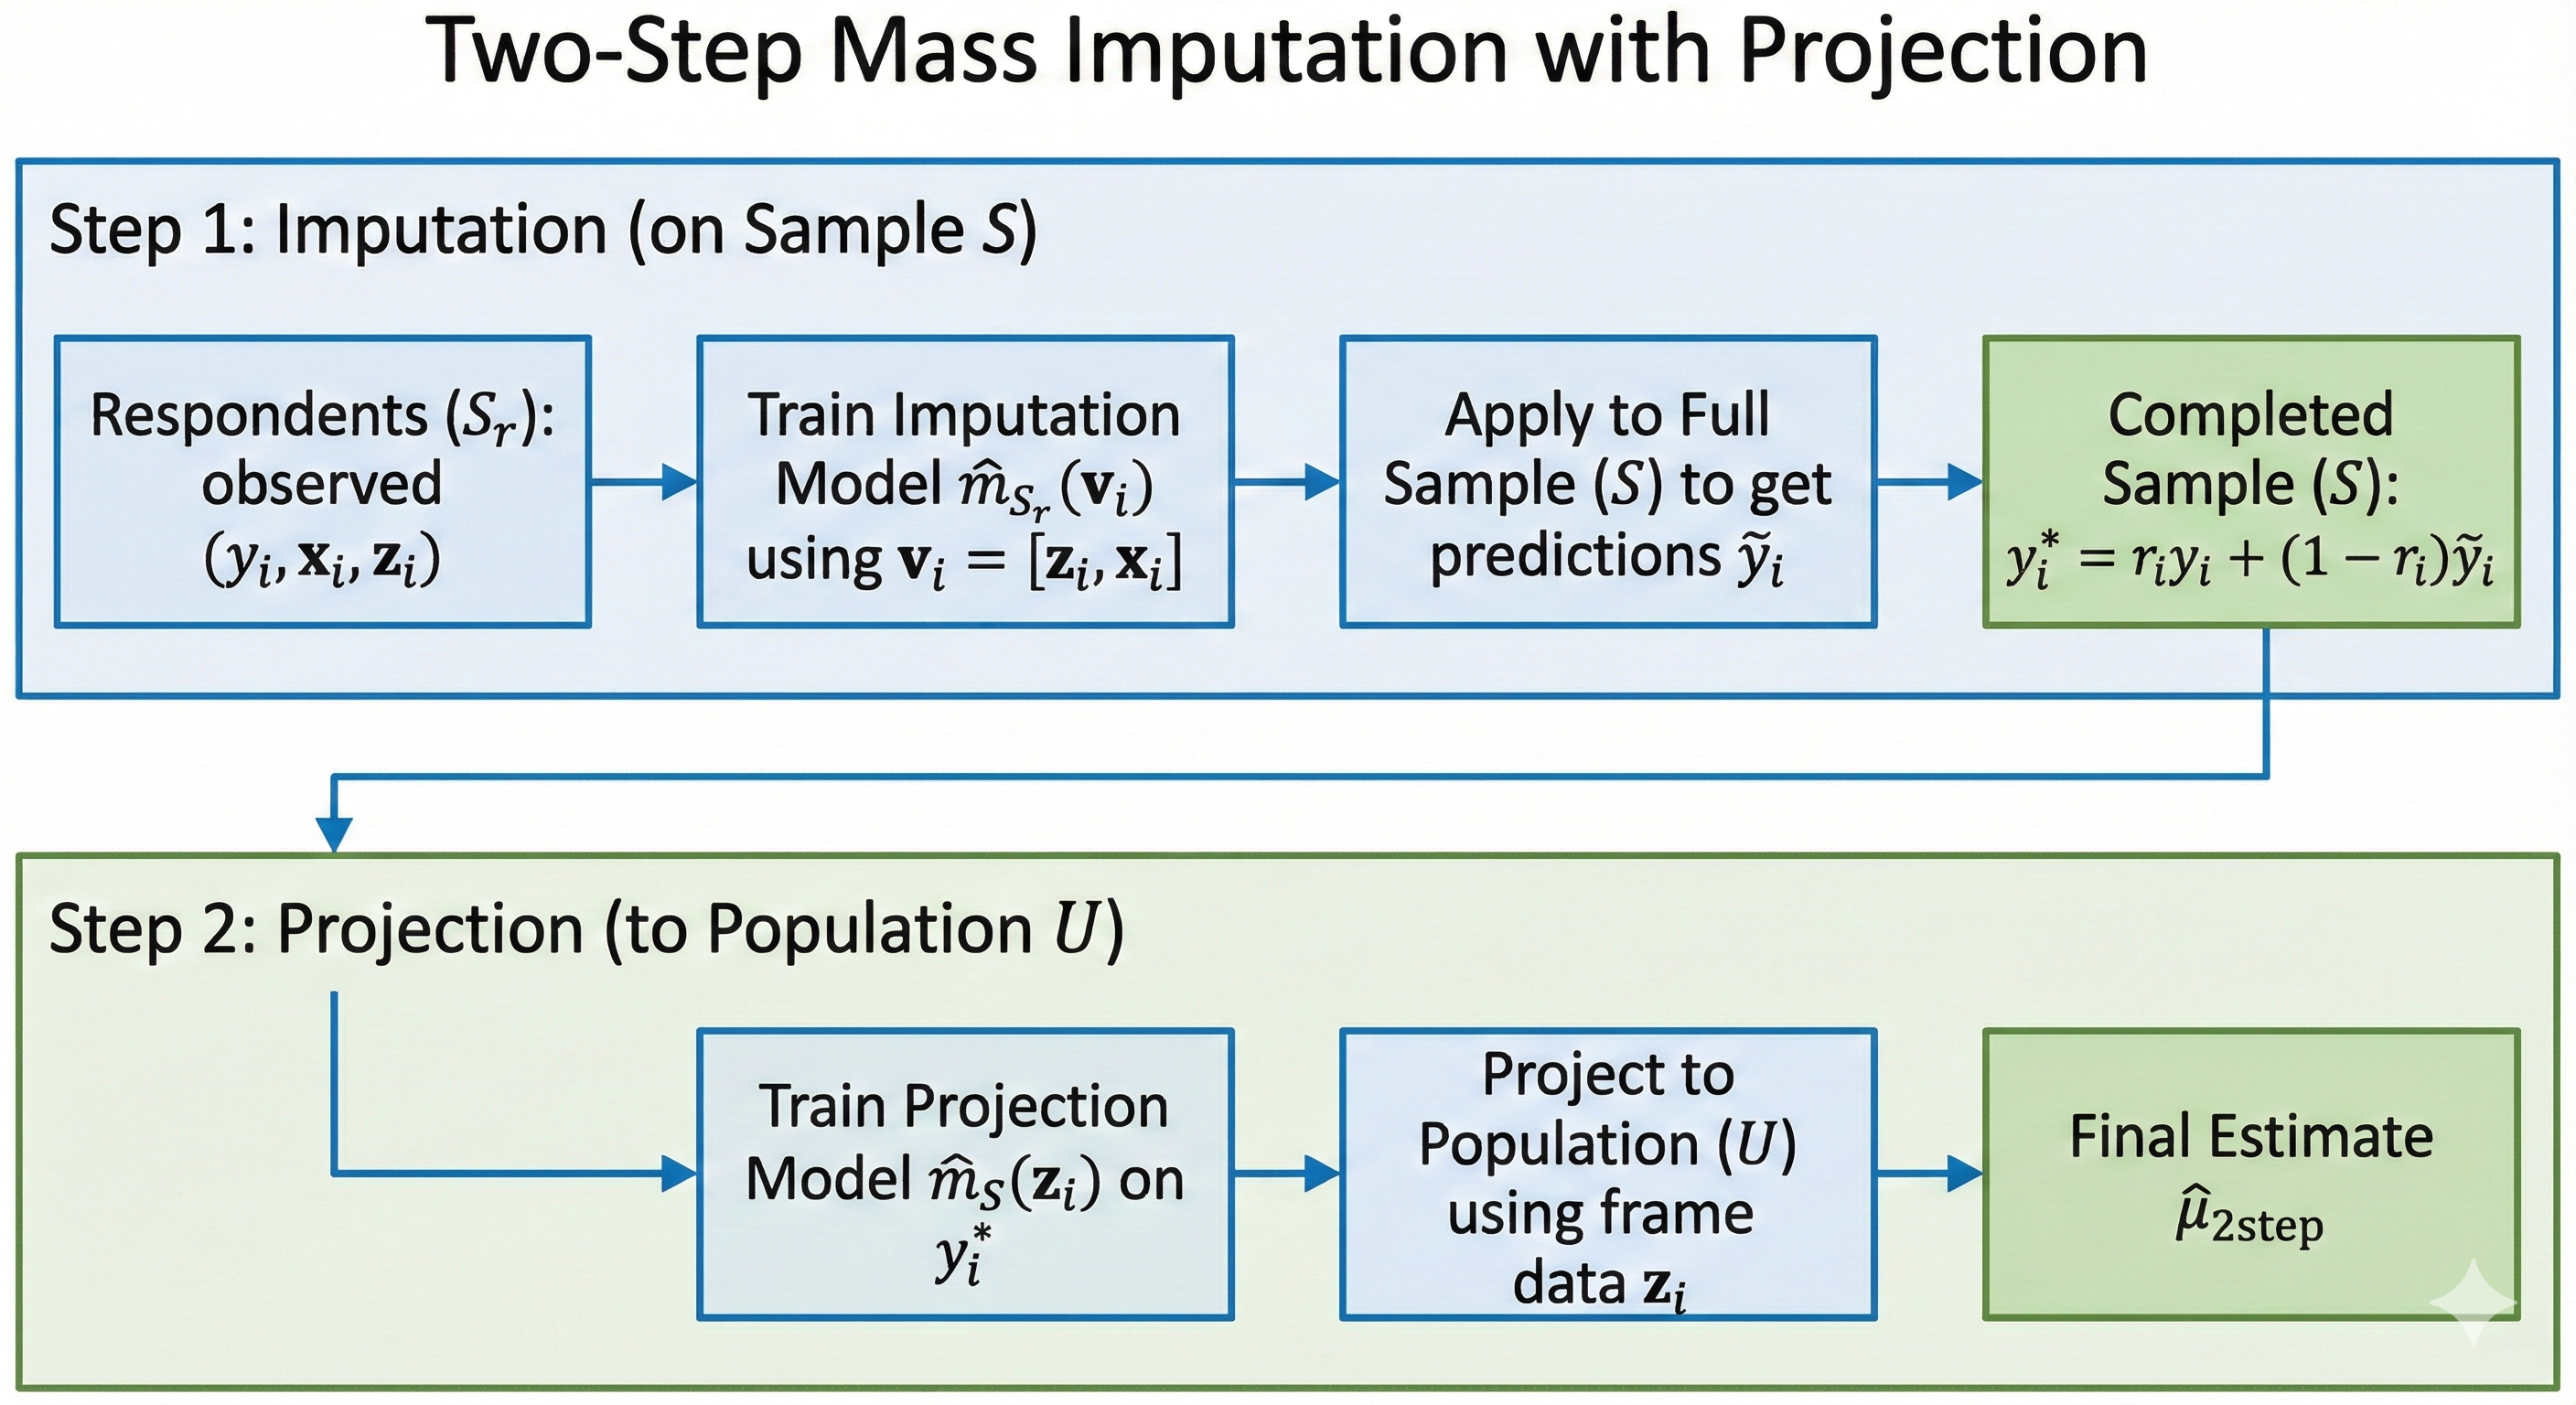
\includegraphics[width=0.8\textwidth]{paper/diagrams/3A.png}

\paragraph{Scenario 4: Historical Data and Pre-Trained Models.}

We consider the specific case where the frame data $\mathbf{z}_i$ consists of outcomes from a previous administrative period ($t-1$), such that $\mathbf{z}_i$ contains $y_i^{(t-1)}$. Additionally, we observe a vector of current-period auxiliary variables $\mathbf{x}_i$ for the sample $S$, which are not available on the frame. In this scenario, we rely on modeling assumptions to handle missingness, reserving propensity score adjustments for the robust framework in Scenario 5. We motivate the proposed estimator by examining the limitations of two preliminary approaches.

The simplest approach, the \textbf{Naive Difference Estimator}, treats the previous period's outcome $y_i^{(t-1)}$ as a direct proxy for the current outcome $y_i$. Because current outcomes are strictly observed for respondents, the adjustment is calculated over the respondent set $S_r$:
\[ 
\hat{\mu}_{\text{diff}} = \bar{Y}^{(t-1)} + \frac{1}{N}\sum_{i\in S_r}\frac{y_i - y_i^{(t-1)}}{\pi_i} 
\]
This estimator is systematically biased because it sums differences only over the respondent set $S_r$, failing to project the change in outcome to the non-responding portion of the population. It fails to utilize $\mathbf{x}_i$ to account for heterogeneous evolution of the variable of interest.

To reduce the variance of the difference estimator, one may employ a \textbf{Pre-trained Difference Estimator}. We utilize a model $f_{\text{hist}}(\mathbf{z}_i)$ trained on historical trends (e.g., $y^{(t-1)} \sim \mathbf{z}^{(t-1)}$) to generate a baseline prediction $\hat{y}_i^{\text{hist}} = f_{\text{hist}}(\mathbf{z}_i)$. The estimator becomes:
\[
\hat{\mu}_{\text{Pre-train}}
= \frac{1}{N} \left(
  \sum_{i \in U} f_{\text{hist}}(\mathbf{z}_i)
  + \sum_{i \in S} \frac{r_i\bigl(y_i - f_{\text{hist}}(\mathbf{z}_i)\bigr)}{\pi_i}
\right),
\]

While this method leverages the frame to reduce the variance of the projection term (the first summand), the bias correction (the second summand) is restricted to the respondent set $S_r$. If the relationship between $y_i$ and $\mathbf{z}_i$ has drifted due to factors associated with $\mathbf{x}_i$, and response depends on $\mathbf{x}_i$, the residual term computed over $S_r$ will be a biased estimate of the population residual.

Finally, we propose the \textbf{Hist-PPD Estimator}, which applies the Mass Imputation framework (Scenario 3) to this temporal context. We retain the historical function $f_{\text{hist}}(\mathbf{z}_i)$ for the population projection. However, to account for systematic evolution captured by current auxiliaries, we replace the observed $y_i$ with the mass-imputed value $y_i^\star = \hat{m}_{S_r}(\mathbf{v}_i)$, derived using the current sample auxiliaries $\mathbf{x}_i$. 

Crucially, because $y_i^\star$ is generated for all sampled units, the residual adjustment is computed over the \textit{full sample} $S$, utilizing the sample design weights to project the residuals to the population:
\[ 
\hat{\mu}_{\text{Hist-PPD}} = \frac{1}{N} \left( \underbrace{\sum_{i \in U} f_{\text{hist}}(\mathbf{z}_i)}_{\text{Population Projection}} + \underbrace{\sum_{i \in S} \frac{y_i^\star - f_{\text{hist}}(\mathbf{z}_i)}{\pi_i}}_{\text{Sample-based Adjustment}} \right) 
\]
This formulation ensures that the historical model provides the primary signal structure, while the mass-imputed residuals correct for temporal drift and bias using the full sample information $S$, rather than the restricted respondent set $S_r$.


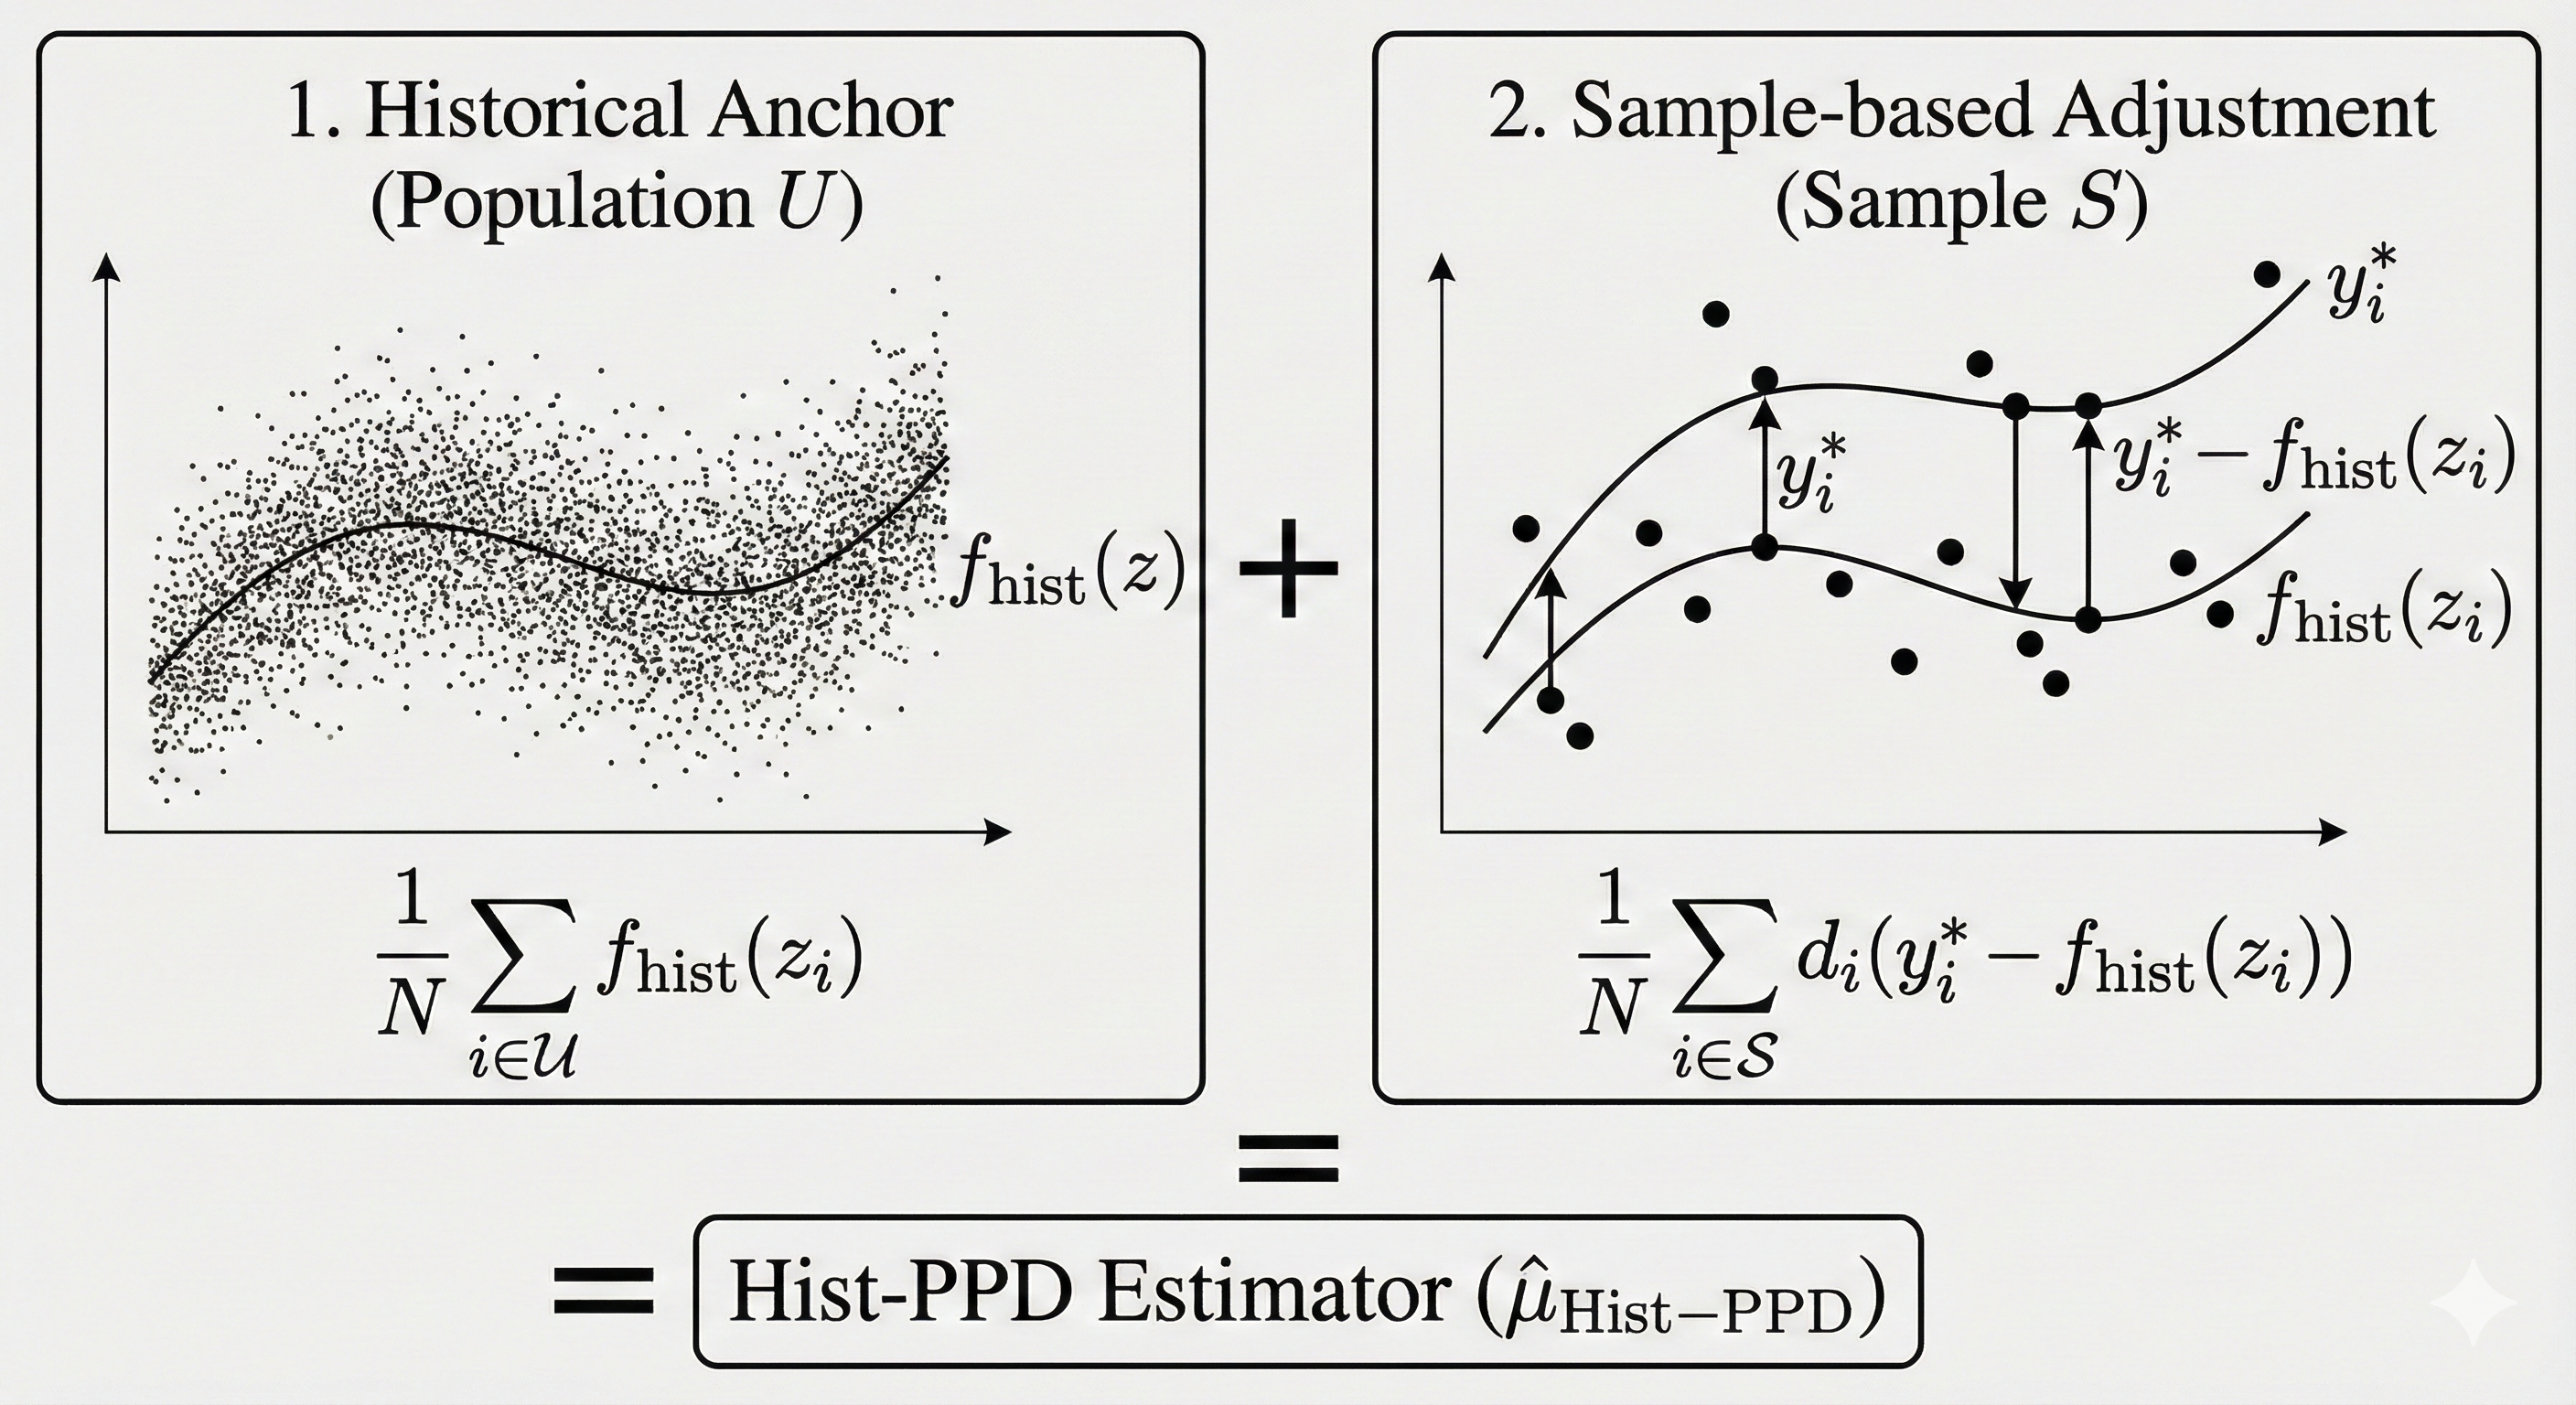
\includegraphics[width=0.8\textwidth]{paper/diagrams/Scenario4.png}


\paragraph{Scenario 5: Robust Integration (The Hist-PPD-DR Estimator).}

While the estimator in Scenario 4 ($\hat{\mu}_{\text{Hist-PPD}}$) incorporates historical anchors and current signals, it relies entirely on the imputation model being correct. To safeguard against model failure (e.g., if the current signal $x_i$ drifts in a way the model misses), we apply a doubly robust correction. This is the \textbf{Hist-PPD-DR} estimator.

This estimator applies the established doubly robust model-calibration framework (e.g., Kim and Rao, 2012) to the historical setting. It augments the mass imputation estimator with an inverse-probability weighting (IPW) correction based on the response propensity $\hat{p}_i$.

\medskip
\noindent\emph{Estimator Formula.}
Let $\tilde{y}_i$ be the predicted value from the imputation model using current signals, and $f_{\text{hist}}(\mathbf{z}_i)$ be the historical projection. The robust estimator is:

\begin{equation}
\hat{\mu}_{\text{Hist-PPD-DR}} = \frac{1}{N} \left( 
    \sum_{i\in U} f_{\text{hist}}(\mathbf{z}_i)
    \;+\; 
    \sum_{i\in S} d_i \Bigl\{\tilde{y}_i - f_{\text{hist}}(\mathbf{z}_i)\Bigr\}
    \;+\; 
    \sum_{i\in S_r} \frac{d_i}{\hat{p}_i}\,\Bigl(y_i - \tilde{y}_i\Bigr)
\right)
\label{eq:Hist-PPD-DR}
\end{equation}

\noindent This can be rearranged into a component form that highlights exactly how each data source contributes to the final estimate:

\[
\hat{\mu}_{\text{Hist-PPD-DR}} = \frac{1}{N} \left( 
    \underbrace{\sum_{i\in U} f_{\text{hist}}(\mathbf{z}_i)}_{\text{Historical Anchor}}
    \;+\; 
    \underbrace{\sum_{i\in S} d_i \Bigl\{\tilde{y}_i - f_{\text{hist}}(\mathbf{z}_i)\Bigr\}}_{\text{Signal Adjustment}}
    \;+\; 
    \underbrace{\sum_{i\in S_r} \frac{d_i}{\hat{p}_i}\Bigl(y_i - \tilde{y}_i\Bigr)}_{\text{Bias Correction}}
\right)
\]

\medskip
\noindent\emph{Derivation.}
We verify the connection between these components by expanding the residual term. For any unit, the robust correction can be rewritten as:
\[
\tilde{y}_i - f_{\text{hist}}(\mathbf{z}_i) + \frac{r_i}{\hat{p}_i}(y_i - \tilde{y}_i) 
= \frac{r_i}{\hat{p}_i}\bigl[y_i - f_{\text{hist}}(\mathbf{z}_i)\bigr] + \Bigl(1-\frac{r_i}{\hat{p}_i}\Bigr)\bigl[\tilde{y}_i - f_{\text{hist}}(\mathbf{z}_i)\bigr]
\]
This reveals that the estimator effectively creates a weighted mixture of the observed residual (from the respondent) and the imputed residual (from the model).

\medskip
\noindent\emph{Properties and Sanity Checks.}
\begin{itemize}
    \item \textbf{Double Robustness:} This estimator is consistent for the population mean if \emph{either}:
    \begin{enumerate}
        \item The outcome model is correct ($E[y_i|\mathbf{x}_i] \approx \tilde{y}_i$), \textbf{OR}
        \item The response propensity model is correct ($\Pr(r_i=1|\mathbf{x}_i) \approx \hat{p}_i$).
    \end{enumerate}
    \item \textbf{Reduction to Scenario 4:} If we ignore the propensity weights (set $\hat{p}_i=1$) and assume the imputation residuals sum to zero, this collapses to the Mass Imputation estimator $\hat{\mu}_{\text{Hist-PPD}}$.
    \item \textbf{Complete Response:} If $r_i \equiv 1$ (no missing data), the bias correction term vanishes, and the estimator collapses to the standard \textbf{GREG/Difference Estimator}.
    \item \textbf{No History:} If $f_{\text{hist}} \equiv 0$, the estimator simplifies to the classic \textbf{AIPW (Doubly Robust)} estimator.
\end{itemize}



\begin{table}[htbp]
\centering
\caption{Comparison of Estimators: Training Data sources, Prediction Targets, and Auxiliary Usage. Note the distinction in Mass Imputation between the model trained on respondents ($\hat{m}_{S_r}$) and the model trained on the completed sample ($\hat{m}_S$).}
\label{tab:estimators_comparison}
\renewcommand{\arraystretch}{1.3} % Adds breathing room between rows
\resizebox{\textwidth}{!}{% Resizes table to fit text width if necessary
\begin{tabular}{@{} l l l l l @{}}
\toprule
\textbf{Estimator} & \textbf{Key Component} & \textbf{Training Set} (Learns $\beta$) & \textbf{Prediction Target} (Gets $\hat{y}$) & \textbf{Auxiliaries Used} \\ 
\midrule

% Row 1: Imputation
\textbf{1. Imputation} & 
$\hat{m}_{S_r}(\mathbf{x}_i)$ & 
Respondents ($S_r$) & 
Missing Sample ($S_m$) & 
Sample ($\mathbf{x}$) \\

% Row 2: NWA
\textbf{2. NWA (IPW)} & 
$\hat{p}_i(\mathbf{v}_i)$ & 
Full Sample $S$ (Response Flag) & 
Respondents ($S_r$) & 
Sample ($\mathbf{x}$) \\

% Row 3: GREG
\textbf{3. Std. GREG} & 
$\hat{m}_{S_r}(\mathbf{z}_i)$ & 
Respondents ($S_r$) & 
Population ($U$) & 
Frame ($\mathbf{z}$) \\

\midrule

% Row 4: Mass Imputation (Split into two steps for clarity)
\textbf{4. Mass Imputation} & & & & \\
\hspace{3mm} \textit{Step 1: Impute} & 
$\hat{m}_{S_r}(\mathbf{v}_i)$ & 
Respondents ($S_r$) & 
Full Sample ($S$) & 
Rich Sample ($\mathbf{x}, \mathbf{z}$) \\
\hspace{3mm} \textit{Step 2: Project} & 
$\hat{m}_{S}(\mathbf{z}_i)$ & 
\textbf{Completed Sample} ($S$) & 
Population ($U$) & 
Frame ($\mathbf{z}$) \\

\midrule

% Row 5: Hist-PPD
\textbf{5. Hist-PPD} & 
$f_{\text{hist}}(\mathbf{z}_i)$ & 
\textbf{Historical Data} ($t-1$) & 
Population ($U$) & 
History ($\mathbf{z}$) \\

% Row 6: Hist-PPD-DR
\textbf{6. Hist-PPD-DR} & 
$f_{\text{hist}}$ + $\hat{m}_{S_r}$ & 
History ($t-1$) \textbf{\&} Respondents ($S_r$) & 
Population ($U$) & 
\textbf{All} ($\mathbf{x}, \mathbf{z}, \text{History}$) \\

\bottomrule
\end{tabular}%
}
\end{table}


% ------------------------------------------------- %
% -------------- MODEL SPECIFICATION -------------- %
% ------------------------------------------------- %
\section{Model Specification}
\label{sec:model_spec}


To implement the Hist-PPD-DR estimator defined in Equation \eqref{eq:PPD-DR-total-E}, we must specify two distinct working models: the outcome model $m_S(\mathbf{v}_i)$ used for mass imputation, and the response probability model $\hat{p}_i(\mathbf{v}_i)$ used for propensity weighting.

Throughout, we adopt the standard Missing at Random (MAR) assumption for item nonresponse: $r_i \perp y_i \mid \mathbf v_i$, where $\mathbf v_i = [\mathbf z_i,\mathbf x_i]$ collects the frame and sample auxiliaries observed for every sampled unit. Under MAR it is not contradictory that the same predictor vector $\mathbf v_i$ drives both the outcome model $m_S(\mathbf v_i)$ used for imputation and the response model $\rho(\mathbf v_i) = \Pr(r_i=1 \mid \mathbf v_i)$ used for weighting. Intuitively, $\mathbf v_i$ is allowed to explain both how large $y_i$ tends to be and how likely unit $i$ is to respond; MAR only rules out any remaining dependence of $r_i$ on the unobserved part of $y_i$ once $\mathbf v_i$ is fixed. This is precisely the setup used in the survey–sampling literature on nonresponse adjustment: doubly robust and model–calibration estimators are built from one regression of $y$ on $\mathbf v_i$ and one regression of $r_i$ on $\mathbf v_i$, fitted on the same set of auxiliaries that are available for all units in the sample (e.g., Little and Rubin, 2002; Kim and Haziza, 2014; Haziza and Beaumont, 2017; Kim and Rao, 2012). In our application, we follow this principle by taking $\mathbf v_i=[\mathbf z_i,\mathbf x_i]$ as the common predictor set for both the XGBoost imputation model and the logistic propensity model.


Recent literature in survey sampling emphasizes that while Double Robustness protects against the misspecification of one model, the finite-sample performance of the estimator depends heavily on the stability and predictive power of these models \parencite{Haziza2017}. Consequently, we adopt a hybrid modeling strategy that leverages the strengths of machine learning for prediction and the stability of parametric estimation for weighting.

\subsection{Imputation Model: Gradient Boosted Trees (XGBoost)}

e
\begin{enumerate}
    \item \textbf{Automatic Interaction Detection:} Unlike linear models, which require explicit specification of interaction terms (e.g., $\mathbf{x}_i \times \mathbf{z}_i$), XGBoost automatically learns complex non-linear interactions between the frame and sample data.
    \item \textbf{Robustness to Skewness:} Survey data often follow heavy-tailed distributions (e.g., Gamma-like revenue data). Tree-based methods are invariant to monotonic transformations of the predictors and are less sensitive to outliers in the covariate space than linear projection methods.
    \item \textbf{Regularization:} XGBoost includes both $L_1$ and $L_2$ regularization terms in its objective function, preventing overfitting even when the number of sample predictors $p_x$ is large relative to the sample size $n$.
\end{enumerate}

\subsection{Propensity Score Model: The Parametric Score Method}

For the propensity score estimation $\hat{p}_i$, we employ a parametric logistic regression model estimated via the \textbf{Score Method} (Maximum Likelihood), rather than a machine learning classifier. While machine learning methods like XGBoost are powerful classifiers, they are often ill-suited for propensity weighting in finite population inference. A known issue with boosting or random forests in this context is ``perfect separation,'' where the model assigns probabilities close to 0 or 1. In a weighting context (Scenario 1 and 3), this results in extreme weights ($\hat{p}_i^{-1}$) that can destabilize the estimator and drastically inflate variance. In contrast, the Score Method (Logistic Regression) provides two critical statistical properties required for robust weighting \parencite{KimHaziza2014}:

\begin{enumerate}
    \item \textbf{Calibration Constraints:} The maximum likelihood estimator $\hat{\boldsymbol{\alpha}}$ for the logistic model solves the score equations:
    \begin{equation}
        \sum_{i \in S} \left( r_i - \frac{1}{1 + \exp(-\mathbf{v}_i^T \boldsymbol{\alpha})} \right) \mathbf{v}_i = \mathbf{0}
    \end{equation}
    This implies that the residuals sum to zero over the sample space. As noted by \parencite{Haziza2017},, this inherent balancing property ensures that the estimated weights effectively align the covariate distributions of the respondents and the sample, a property not guaranteed by standard machine learning classifiers.
    
    \item \textbf{Boundedness:} The logistic link function produces smooth probabilities strictly bounded away from 0 and 1 (assuming no complete separation), resulting in a more stable distribution of weights and lower variance for the final estimator.
\end{enumerate}

Therefore, our simulation utilizes XGBoost for $m_S(\cdot)$ to maximize predictive accuracy, and Logistic Regression for $\rho(\cdot)$ to ensure stability and calibration of the weights.




% ------------------------------------------------- %
% ------------------- NEW SECTION ------------------- %
% ------------------------------------------------- %

%% Variance estimation
\section{Variance Estimation}

A major challenge in using the estimator proposed in Scenario 3 is variance estimation. Standard variance formulas (e.g., Horvitz-Thompson variance) treat the completed values $y_i^\star$ as if they were observed values. This leads to the ``naive variance estimation'' problem, where the uncertainty associated with the imputation model $\hat{m}_{S_{r}}(\cdot)$ is ignored, resulting in standard errors that are too small and confidence intervals that have poor coverage (Kim and Rao, 2012).

To properly account for both the sampling design and the uncertainty in the imputation mechanism, we recommend a replication-based approach, specifically the bootstrap.

\paragraph{The Bootstrap for Mass Imputation.}
To estimate the variance of our estimators, we employ a bootstrap procedure that captures the variability of the model fitting process. The procedure is as follows:

\begin{enumerate}
    \item \textbf{Generate Replicates:} Draw $B$ bootstrap samples $S^{(b)}$ from the original sample $S$ using the design weights (e.g., using the rescaling bootstrap for complex designs).
    \item \textbf{Re-Impute:} For each bootstrap sample $b = 1, \dots, B$:
    \begin{itemize}
        \item Refit the imputation model $\hat{m}_{S_{r}}^{(b)}(\mathbf{v}_i)$ using only the respondents in the bootstrap replicate $S_r^{(b)}$.
        \item Generate new imputed values $\tilde{y}_i^{(b)}$ for the non-respondents in that replicate.
        \item Refit the projection model $\hat{m_S}^{(b)}(\mathbf{z}_i)$ on the completed bootstrap sample (unless utilizing a fixed historical model $f_{\text{hist}}$, which remains constant).
    \end{itemize}
    \item \textbf{Calculate Estimate:} Compute the estimator $\hat{\mu}^{(b)}$ for each replicate.
\end{enumerate}

The variance estimator is then the empirical variance of the $B$ bootstrap estimates:
\[
\widehat{V}(\hat{\mu}_{\text{PPD-DR}}) = \frac{1}{B-1} \sum_{b=1}^B \left( \hat{\mu}^{(b)} - \bar{\hat{\mu}} \right)^2
\]
where $\bar{\hat{\mu}}$ is the mean of the bootstrap replicates. This method is asymptotically consistent and automatically captures the additional variance introduced by the imputation and projection steps.






\section{Simulation}
\todo[inline, color=orange]{NEED TO VALIDATE/VERIFY - THINK HARD ABOUT THIS!}

To evaluate the finite-sample performance of the proposed estimation strategy, we conduct a comprehensive simulation study. We follow the standard evaluation framework for missing data estimators in survey sampling (e.g., Kim and Rao, 2012; Haziza and Beaumont, 2017). Our primary objective is to study and benchmark the estimators against each other under realistic conditions where historical administrative data is ubiquitous, but current sample data is subject to non-response.

\subsection{Simulation Setup}
We employ a four-step data generation process to create a finite population, draw samples, induce non-response, and compute estimates. We repeat this process $K=2,000$ times to approximate the sampling distribution of the estimators.

\paragraph{Data Generation Process.}
We generate a finite population $U$ of size $N=10,000$. Following the simulation designs of Haziza and Beaumont (2017), we utilize Gamma distributions to mimic the right-skewed nature of business survey data (e.g., revenue or production).

\begin{itemize}
    \item \textbf{Historical Administrative Data ($z_i$):} 
    We generate a historical variable $z_i$ (representing, for example, previous census revenue) from a Gamma distribution with shape $\alpha=2$ and scale $\beta=10$:
    \[ z_i \sim \text{Gamma}(2, 10) \]
    This results in a strictly positive, right-skewed distribution with a mean of 20, typical of economic populations.
    
    \item \textbf{Current Signal ($x_i$):} 
    We generate the current signal $x_i$ (e.g., a real-time auxiliary signal) as a function of the history, subject to drift. We use an additive error structure with a positive distribution to ensure $x_i$ remains strictly positive:
    \[ x_i = 0.8 z_i + \epsilon_{x,i} \]
    where $\epsilon_{x,i} \sim \text{Exponential}(5)$. This creates a strong positive correlation ($\rho \approx 0.7$) between the past and present, reflecting a stable but evolving population.
    
    \item \textbf{Outcome Variable ($y_i$):} 
    We generate the current outcome of interest $y_i$ as a function of both the historical anchor and the current signal:
    \[ y_i = 2 + 0.5 z_i + 1.5 x_i + \epsilon_{y,i} \]
    where $\epsilon_{y,i} \sim N(0, 5)$. This setup ensures that while history ($z_i$) is predictive, the current signal ($x_i$) contains unique, necessary information to capture the true outcome.
    
    \item \textbf{Sampling ($S$):} 
    From the population, we draw a probability sample $S$ of size $n=500$ using Simple Random Sampling (SRS).
    
    \item \textbf{Non-response ($r_i$):} 
    We introduce item non-response using a logistic propensity model. To simulate informative missingness often found in business surveys (where unit size affects response behavior), we model the response probability as a function of the current signal $x_i$:
    \[ \text{logit}(\Pr(r_i=1)) = -1 + 0.1 x_i \]
    This induces a Missing at Random (MAR) mechanism. Crucially, because response depends on $x_i$, and $y_i$ depends on $x_i$, the observed set of respondents is systematically biased. Estimators that fail to account for $x_i$ will therefore yield biased inference.
\end{itemize}


\subsection{Evaluation Metrics}

We assess the performance of each estimator using three standard statistical metrics. Let $\hat{\theta}_k$ be the estimate from the $k$-th simulation run and $\theta$ be the true population total.

We measure systematic error using Relative Bias (RB). Values close to 0\% indicate unbiasedness; generally, an absolute relative bias greater than 5\% is considered problematic in official statistics.
\[ \text{RB}(\hat{\theta}) = \frac{1}{K} \sum_{k=1}^{K} \left( \frac{\hat{\theta}_k - \theta}{\theta} \right) \times 100\% \]

We measure efficiency using Relative Root Mean Square Error (RRMSE), which captures the combined effect of bias and variance.
\[ \text{RRMSE}(\hat{\theta}) = \sqrt{ \frac{1}{K} \sum_{k=1}^{K} \left( \frac{\hat{\theta}_k - \theta}{\theta} \right)^2 } \times 100\% \]

Finally, we evaluate uncertainty quantification using the Coverage Rate (CR), 
\[ \text{CR} = \frac{1}{K} \sum_{k=1}^{K} \mathbbm{1}\{ \theta \in [\hat{\theta}_k \pm 1.96 \sqrt{\widehat{V}_k}] \} \]
defined as the proportion of simulation runs where the 95\% confidence interval contains the true population value. A valid estimator should have a coverage rate close to 95\%.

\subsection{Comparisons}

We compare five distinct estimators to isolate the contributions of historical data, current signals, and robust corrections:

\begin{enumerate}
    \item \textbf{Naive Estimator:} The standard Horvitz-Thompson estimator using only the respondents $S_r$. It ignores missingness and makes no use of auxiliary data.
    \item \textbf{Weighting Only (NWA):} The standard IPW estimator that adjusts for non-response using propensity scores $\hat{p}_i(x_i, z_i)$, but utilizes no outcome modeling (Scenario 1).
    \item \textbf{Standard Hist-GREG:} The classical generalized regression estimator using only historical data $z_i$ for the projection. It ignores the rich current signals $x_i$ inside the imputation model (Scenario 2).
    \item \textbf{Mass Imputation (Two-Step):} The projection estimator that uses current signals $x_i$ to impute missing values, but lacks the propensity score correction for double robustness (Scenario 3, also the Hist-PPD).
    
    
    \item \textbf{Hist-PPD-DR:} The proposed approach which integrates all available information. It uses $z_i$ for the population anchor, $x_i$ for mass imputation, and propensity weights for residual bias correction.
\end{enumerate}



\newpage
\begin{table}[htbp]
\centering
\scriptsize
\renewcommand{\arraystretch}{2.0}
\caption{Comprehensive Summary of Estimators for Item Nonresponse (Finite-Population Total)}
\label{tab:comprehensive_estimators}

\resizebox{\textwidth}{!}{%
\begin{tabular}{@{} p{2.5cm} p{5.5cm} p{1.5cm} p{2.2cm} p{3.0cm} p{2.5cm} @{}}
\toprule
\textbf{Estimator} & 
\textbf{Formula} ($\widehat{T}$) & 
\textbf{Respon-dents Only?} & 
\textbf{Model Required} & 
\textbf{Assumptions for Consistency} & 
\textbf{Key References} \\ 
\midrule

% 1. Naive
\textbf{Naïve} & 
$\displaystyle \widehat{T}_{\text{naive}} = \frac{N}{\sum_{j \in S_r} d_j} \sum_{i \in S_r} d_i y_i$ & 
Yes & 
None & 
MCAR & 
Cochran (1977); Little \& Rubin (2002) \\

% 2. NWA / Propensity Weighting
\textbf{Propensity Weighting (NWA)} & 
$\displaystyle \widehat{T}_{\text{NWA}} = \sum_{i \in S_r} \frac{d_i}{\hat{p}_i} y_i$ & 
Yes & 
Response $\hat{p}(\mathbf{v})$ & 
MAR, Positivity, Correct $\hat{p}$ & 
Little (1986); Kott (1994); Robins et al. (1994) \\

% 3. Calibration / GREG
\textbf{Calibration / GREG} & 
$\displaystyle \widehat{T}_{\text{reg}} = \sum_{i \in U} f(\mathbf{z}_i) + \sum_{i \in S_r} \frac{d_i}{\hat{p}_i} (y_i - f(\mathbf{z}_i))$ \newline
\textit{(Note: Standard GREG often assumes $\hat{p}_i=1$)} & 
Yes & 
Outcome $f(\mathbf{z})$ & 
Aux $\mathbf{z}$ predictive of $y$; Either correct $f(\mathbf{z})$ OR correct $\hat{p}$ & 
Deville \& Särndal (1992); Särndal \& Lundström (2005) \\

% 4. Imputation
\textbf{Imputation Estimator} & 
$\displaystyle \widehat{T}_{\text{imp}} = \sum_{i \in S_r} d_i y_i + \sum_{i \in S_m} d_i \tilde{y}_i$ \newline
\textit{where $\tilde{y}_i = \hat{m}(\mathbf{v}_i)$} & 
No & 
Outcome $\hat{m}(\mathbf{v})$ & 
MAR, Correct $\hat{m}(\mathbf{v})$ & 
Haziza (2009); Kim \& Fuller (2004) \\

% 5. Doubly Robust (AIPW)
\textbf{Doubly Robust (AIPW)} & 
$\displaystyle \widehat{T}_{\text{DR}} = \sum_{i \in S} d_i \tilde{y}_i + \sum_{i \in S_r} \frac{d_i}{\hat{p}_i} (y_i - \tilde{y}_i)$ & 
No & 
$\hat{m}(\mathbf{v})$ and $\hat{p}(\mathbf{v})$ & 
MAR, Positivity, \textbf{Either} model correct & 
Robins et al. (1994); Kim \& Haziza (2014) \\

% 6. Multiply Robust
\textbf{Multiply Robust (MR)} & 
$\displaystyle \widehat{T}_{\text{MR}} = \sum_{i \in S_r} d_i y_i + \sum_{i \in S_m} d_i \tilde{y}_i^{\text{MR}}$ & 
No & 
Multiple models & 
\textbf{Any one} model correct & 
Chen \& Haziza (2017); Han (2014) \\

% 7. Hist-PPD-DR (The paper's proposed estimator)
\textbf{Hist-PPD-DR} & 
$\displaystyle \widehat{T}_{\text{PPD-DR}} = \sum_{i \in U} f(\mathbf{z}_i) + \sum_{i \in S} d_i (\tilde{y}_i - f(\mathbf{z}_i)) + \sum_{i \in S_r} \frac{d_i}{\hat{p}_i} (y_i - \tilde{y}_i)$ & 
No & 
$f(\mathbf{z})$, $\hat{m}(\mathbf{v})$, $\hat{p}(\mathbf{v})$ & 
MAR, Positivity, \textbf{Either} $\hat{m}$ or $\hat{p}$ correct (given fixed $f$) & 
Kim \& Haziza (2014); Särndal \& Lundström (2005) \\

\bottomrule
\end{tabular}%
}
\end{table}


\includegraphics[width=0.8\textwidth]{paper/diagrams/MissingData.png}